\documentclass[12pt,reqno,oneside]{amsart}
\usepackage{import}
\usepackage{hyperref}
%===============================%
%  Packages and basic settings  %
%===============================%
\usepackage[headheight=15pt,rmargin=0.5in,lmargin=0.5in,tmargin=0.75in,bmargin=0.75in]{geometry}
\usepackage{fancyhdr}
\usepackage{imakeidx}
\usepackage{framed}
\usepackage{amssymb}
\usepackage{amsmath}
\usepackage{mathrsfs}
\usepackage{enumitem}
\usepackage{multirow}
\usepackage{hyperref}
\usepackage[capitalise,noabbrev]{cleveref}
\usepackage{appendix}
\usepackage[hyperref,amsthm,amsmath,thref,framed,thmmarks]{ntheorem}
\usepackage{tikz}
\usepackage{tikz-cd}
\usepackage{nomencl}\makenomenclature
\usetikzlibrary{braids,arrows,decorations.markings,calc}

%=======================%
%  Book style settings  %
%=======================%
\pagestyle{fancy}
\fancyhf{}
\fancyhead[L]{\nouppercase{\leftmark}}
\fancyfoot[C]{\thepage}
\setlength\parindent{0pt}
\raggedbottom

%====================================%
%  Theorems, environments & cleveref  %
%====================================%
\theoremstyle{plain}\newtheorem{theorem}{Theorem}[section]
\theoremstyle{nonumberplain}\renewtheorem{theorem*}{Theorem}
\theoremstyle{plain}\newtheorem{proposition}[theorem]{Proposition}
\theoremstyle{nonumberplain}\renewtheorem{proposition*}{Proposition}
\theoremstyle{plain}\newtheorem{corollary}[theorem]{Corollary}
\theoremstyle{nonumberplain}\renewtheorem{corollary*}{Corollary}
\theoremstyle{plain}\newtheorem{lemma}[theorem]{Lemma}
\theoremstyle{nonumberplain}\renewtheorem{lemma*}{Lemma}
\theoremstyle{plain}\newtheorem{conjecture}[theorem]{Conjecture}
\theoremstyle{nonumberplain}\renewtheorem{conjecture*}{Conjecture}
\theoremstyle{plain}\newtheorem{remark}[theorem]{Remark}
\theoremstyle{nonumberplain}\renewtheorem{remark*}{Remark}
\theoremstyle{plain}\newtheorem{problem}[theorem]{Open Problem}
\theoremstyle{nonumberplain}\renewtheorem{problem*}{Open Problem}
\theoremstyle{plain}\newtheorem{heuristic}[theorem]{Heuristic}
\theoremstyle{nonumberplain}\renewtheorem{heuristic*}{Heuristic}
\crefname{conjecture}{Conjecture}{Conjectures}

\newenvironment{stabular}[2][1]
  {\def\arraystretch{#1}\tabular{#2}}
  {\endtabular}

%==================================%
%  Custom commands & environments  %
%==================================%
\newcommand{\legendre}[2]{\left(\frac{#1}{#2}\right)}
\newcommand{\dlegendre}[2]{\displaystyle{\left(\frac{#1}{#2}\right)}}
\newcommand{\tlegendre}[2]{\textstyle{\left(\frac{#1}{#2}\right)}}
\newcommand{\psum}{\sideset{}{'}\sum}
\newcommand{\asum}{\sideset{}{^{\ast}}\sum}
\newcommand{\tmod}[1]{\ (\mathrm{mod}\text{ }#1)}
\renewcommand{\bmod}[1]{\ \left(\mathrm{mod}\text{ }#1\right)}
\newcommand{\xto}[1]{\xrightarrow{#1}}
\newcommand{\xfrom}[1]{\xleftarrow{#1}}
\newcommand{\normal}{\mathrel{\unlhd}}
\newcommand{\mf}{\mathfrak}
\newcommand{\mc}{\mathcal}
\newcommand{\ms}{\mathscr}

\newcommand{\Mat}{\mathrm{Mat}}
\newcommand{\GL}{\mathrm{GL}}
\newcommand{\SL}{\mathrm{SL}}
\newcommand{\PSL}{\mathrm{PSL}}
\renewcommand{\O}{\mathrm{O}}
\newcommand{\SO}{\mathrm{SO}}
\newcommand{\U}{\mathrm{U}}
\newcommand{\Sp}{\mathrm{Sp}}

\newcommand{\N}{\mathbb{N}}
\newcommand{\Z}{\mathbb{Z}}
\newcommand{\Q}{\mathbb{Q}}
\newcommand{\R}{\mathbb{R}}
\newcommand{\C}{\mathbb{C}}
\newcommand{\F}{\mathbb{F}}
\renewcommand{\H}{\mathbb{H}}
\renewcommand{\P}{\mathbb{P}}

\renewcommand{\a}{\alpha}
\renewcommand{\b}{\beta}
\newcommand{\g}{\gamma}
\renewcommand{\d}{\delta}
\newcommand{\z}{\zeta}
\renewcommand{\t}{\theta}
\renewcommand{\i}{\iota}
\renewcommand{\k}{\kappa}
\renewcommand{\l}{\lambda}
\newcommand{\s}{\sigma}
\newcommand{\w}{\omega}

\newcommand{\G}{\Gamma}
\newcommand{\D}{\Delta}
\renewcommand{\L}{\Lambda}
\newcommand{\W}{\Omega}
\newcommand{\scL}{\mathscr{L}}

\newcommand{\e}{\varepsilon}
\newcommand{\vt}{\vartheta}
\newcommand{\vphi}{\varphi}
\newcommand{\emt}{\varnothing}

\newcommand{\x}{\times}
\newcommand{\ox}{\otimes}
\newcommand{\op}{\oplus}
\newcommand{\bigox}{\bigotimes}
\newcommand{\bigop}{\bigoplus}
\newcommand{\del}{\partial}
\newcommand{\<}{\langle}
\renewcommand{\>}{\rangle}
\newcommand{\lf}{\lfloor}
\newcommand{\rf}{\rfloor}
\newcommand{\wtilde}{\widetilde}
\newcommand{\what}{\widehat}
\newcommand{\conj}{\overline}
\newcommand{\cchi}{\conj{\chi}}

\DeclareMathOperator{\id}{\textrm{id}}
\DeclareMathOperator{\sgn}{\mathrm{sgn}}
\DeclareMathOperator{\im}{\mathrm{im}}
\DeclareMathOperator{\rk}{\mathrm{rk}}
\DeclareMathOperator{\adj}{\mathrm{adj}}
\DeclareMathOperator{\tr}{\mathrm{trace}}
\DeclareMathOperator{\nm}{\mathrm{norm}}
\DeclareMathOperator{\disc}{\mathrm{disc}}
\DeclareMathOperator{\ord}{\mathrm{ord}}
\DeclareMathOperator{\sym}{\mathrm{sym}}
\DeclareMathOperator{\ext}{\mathrm{ext}}
\DeclareMathOperator{\Hom}{\mathrm{Hom}}
\DeclareMathOperator{\End}{\mathrm{End}}
\DeclareMathOperator{\Aut}{\mathrm{Aut}}
\DeclareMathOperator{\Tor}{\mathrm{Tor}}
\DeclareMathOperator{\Ann}{\mathrm{Ann}}
\DeclareMathOperator{\Gal}{\mathrm{Gal}}
\DeclareMathOperator{\Trace}{\mathrm{Tr}}
\DeclareMathOperator{\Norm}{\mathrm{N}}
\DeclareMathOperator{\Cl}{\mathrm{Cl}}
\DeclareMathOperator{\Span}{\mathrm{Span}}
\DeclareMathOperator*{\Res}{\mathrm{Res}}
\DeclareMathOperator{\Vol}{\mathrm{Vol}}
\DeclareMathOperator{\Li}{\mathrm{Li}}
\DeclareMathOperator{\Supp}{\mathrm{Supp}}
\renewcommand{\Re}{\mathrm{Re}}
\renewcommand{\Im}{\mathrm{Im}}
\DeclareMathOperator{\Ph}{\mathrm{Ph}}
\DeclareMathOperator{\SC}{\mathrm{SC}}


\newcommand{\GH}{\G\backslash\H}
\newcommand{\GG}{\G_{\infty}\backslash\G}

\newenvironment{psmallmatrix}
  {\left(\begin{smallmatrix}}
  {\end{smallmatrix}\right)}

\newcommand{\smc}[1]{
    \mathchoice
    {{\scriptstyle\mathcal{#1}}}
    {{\scriptstyle\mathcal{#1}}}
    {{\scriptscriptstyle\mathcal{#1}}}
    {\scalebox{0.7}{$\scriptscriptstyle\mathcal{#1}$}}
}

%============%
%  Comments  %
%============%
\newcommand{\todo}[1]{\textcolor{red}{\sf Todo: [#1]}}

%===================%
%  Label reminders  %
%===================%
% [label=(\roman*)]
% [label=(\alph*)]
% [label=(\arabic{enumi})]

%==================%
%  Other settings  %
%==================%
\pgfdeclarelayer{background}
\pgfsetlayers{background,main}
\tikzset{->-/.style={decoration={
  markings,
  mark=at position .5 with {\arrow{>}}},postaction={decorate}}}

%=================%
%  Title & Index  %
%=================%
\title{Research Statement}
\author{Henry Twiss}
\date{\today}
\makeindex

\begin{document}

\maketitle

\textbf{Background}: I am interested in studying the simultaneous non-vanishing of products of elliptic $L$-functions with quadratic conductor over function fields and twisted by quadratic Dirichlet characters, namely $L(s_{1},E_{1} \x \chi_{d})L(s_{2},E_{2} \x \chi_{d})$, at the central value $s = \frac{1}{2}$. This will be accomplished by leveraging the properties of Weyl group multiple Dirichlet series. The \textit{function field} $\F_{q}(t)$ is the field of rational functions in the variable $t$ with coefficients in the finite field $\F_{q}$ of $q$ elements. An \textit{elliptic curve} $E$ over $\F_{q}(t)$ is the set of solutions $(x,y)$ to the cubic equation
\[
  y^{2} = x^{3}+ax+b,
\]
where $a,b \in \F_{q}(t)$. A \textit{quadratic Dirichlet character} $\chi_{d}$, with $d \in \F_{q}[t]$, is a $d$-periodic multiplicative function whose non-zero values are $\pm1$. The \textit{elliptic $L$-function}
\[
  L(s,E \x \chi_{d}) = \sum_{n \ge 1}\frac{a(n)\chi(n)}{n^{s}} = \prod_{p}(1-a(p)p^{-s}+\chi(p)p^{-2s})^{-1},
\]
where the $a(n)$ are certain coefficients defined in terms of the solutions of $E$ modulo $p$, is a complex function initially defined for $\Re(s) > 1$ that encodes the arithmetic information about the elliptic curve $E$ and quadratic Dirichlet character $\chi_{d}$ analytically into itself. It satisfies an Euler products, a functional equation as $s \to 1-s$, and other regularity properties. The \textit{conductor} of $L(s,E \x \chi_{d})$ is a polynomial $N \in \F_{q}[t]$ (depending only upon $E$) such that the functional equation takes shape
\[
  L(s,E \x \chi_{d}) \to |Nd|^{1-2s}L(1-s,E \x \chi_{d}).
\]
Studying the arithmetic information of $E$ is then amenable to understanding the analytic properties of $L(s,E \x \chi_{d})$. Similarly, there are the $L$-functions $L(s,E)$ and $L(s,\chi_{d})$.

A \textit{root system} $\Phi$ is a finite subset of vectors, called \textit{roots}, in some Euclidean vector space $V$ that is invariant under the action of reflections defined by hyperplanes orthogonal to the roots. The invariant subset of reflections is called the \textit{Weyl group} $W$ of $\Phi$. The \textit{Dynkin diagram} of $\Phi$ is a graph completely encoding the properties of $\Phi$. The \textbf{weights} are the set of vectors whose inner product with the roots are integral.

\textbf{Proposal}: The idea of studying arithmetic objects by investigating the arithmetic properties of $L$-functions has its roots traced back to Dirichlet and the Riemann zeta function. In the setting of elliptic curves, there is the infamous Birch–Swinnerton-Dyer conjecture which claims that the rank of $E$ is equal to the order of vanishing of $L(s,E)$ at the special value $s = 1$. It is expected that any $L$-function only vanishes for either trivial or very good reasons at the special values $s = \frac{1}{2}$ and $s = 1$. Simultaneous non-vanishing results are those which state that many $L$-functions do not vanish at a special value. Complex analytic techniques combined with simultaneous non-vanishing results allow for the analytic non-vanishing information to be translated into arithmetic information leading to often astounding results. For example, non-vanishing at $s = 1$ well-known to be closely connected to classical problems such as primes in arithmetic progressions and prime number theorems (see \cite{M}) while non-vanishing at $s = \frac{1}{2}$ is related to the non-vanishing of theta lifting and the nonexistence of Landau–Siegel zeros (see \cite{Da}). These applications are responsible for simultaneous non-vanishing drawing much attention in recent years.

An idea arose in the 1980's that studying an average over a family of $L$-functions would provide insight about each individual $L$-function in the family. The first instance of this construction was introduced by Goldfeld-Hoffstein in \cite{GH}. They averaged over the family of quadratic Dirichlet $L$-functions to construct a multiple Dirichlet series roughly of shape
\[
  Z(s,w) = \sum_{d}\frac{L(s,\chi_{d})P_{d}(s)}{|d|^{w}} = \sum_{m}\frac{L(w,\chi_{m})P_{m}(w)}{|m|^{s}},
\]
where $P_{d}(s)$ are certain explicit correction polynomials possessing functional equations of shape $s \to 1-s$. Variations of this series have been vastly studied throughout the years (see \cite{BW} for a collection of such papers). The multiple Dirichlet series inherits functional equations as $s \to 1-s$ and $w \to 1-w$ from those of $L(s,\chi_{d})$ and $L(w,\chi_{m})$. Composing these functional equations, $Z(s,w)$ satisfies a group of functional equations that is isomorphic to the Weyl group of an $A_{2}$ type root system. This group is isomorphic to the symmetric group $S_{3}$ (the symmetries of a triangle). By successively applying the functional equations, $Z(s,w)$ admits analytic continuation to $\C^{2}$ with a pole at $w = 1$. Taking the residue of $Z\left(\frac{1}{2},w\right)$ at $w = 1$ and applying a contour integral roughly yields an asymptotic of shape
\begin{equation}\label{equ:asymptotic}
  \sum_{|d| \ll X}L\left(\frac{1}{2},\chi_{d}\right)P_{d}\left(\frac{1}{2}\right) = AX\log(X)+BX+o(X),
\end{equation}
for some nonzero constants $A$ and $B$. This implies simultaneous non-vanishing for infinitely many quadratic Dirichlet $L$-functions $L(s,\chi_{d})$ at the central value $s = \frac{1}{2}$. A similar procedure can be done for elliptic $L$-functions. \textbf{I will prove simultaneous non-vanishing for the product of two elliptic $L$-functions with quadratic conductor twisted by quadratic Dirichlet characters over function fields at the central value $s = \frac{1}{2}$. Precisely, for any two elliptic curves $E_{1}$ and $E_{2}$ over $\F_{q}(t)$, there exists infinitely many $d \in \F_{q}[t]$ such that
\[
  L\left(\frac{1}{2},E_{1} \x \chi_{d}\right)L\left(\frac{1}{2},E_{2} \x \chi_{d}\right) \neq 0.
\]}

\textbf{The Strategy}: The underlying idea is to construct a multiple Dirichlet series of shape
\[
  Z(s_{1},s_{2},s_{3}) = \sum_{d}\frac{L(s_{1},E_{1} \x \chi_{d})L(s_{2},E_{2} \x \chi_{d})P_{d}(s_{1},s_{2};E_{1},E_{2})}{|d|^{s_{3}}},
\]
for some correction polynomials $P_{d}(s_{1},s_{2};E_{1},E_{2})$ and show that this series admits analytic continuation to a region containing the point $\left(\frac{1}{2},\frac{1}{2},1\right)$ with a pole at $s_{3} = 1$. Similar analytic techniques to those for $Z(s,w)$ just discussed can be applied to obtain the simultaneous non-vanishing. Therefore, the key insight is \textbf{the analytic continuation of $Z(s_{1},s_{2},s_{3})$ to a suitably large enough domain}. The continuation of $Z$ mimics that of the multiple Dirichlet series
\[
  Z_{\chi}(s_{1},\ldots,s_{5}) = \sum_{d}\frac{\prod_{1 \le i \le 4}L(s_{i},\chi_{d})P_{d}(s_{1},\ldots,s_{4})}{|d|^{s_{5}}},
\]
where $P_{d}(s_{1},\ldots,s_{4})$ are certain correction polynomials. The group of functional equations possessed by $Z_{\chi}$ is an infinite Weyl group isomorphic to the affine dihedral group $\wtilde{D_{4}}$. The associated root system is $\wtilde{D_{4}}$ whose Dynkin diagram is the following:

\begin{center}
  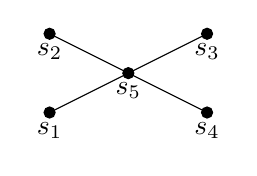
\begin{tikzpicture}
    \node at (-1,-0.5) [below] {$s_{1}$};
    \node at (-1,0.5) [below] {$s_{2}$};
    \node at (0,0) [below] {$s_{5}$};
    \node at (1,-0.5) [below] {$s_{4}$};
    \node at (1,0.5) [below] {$s_{3}$};
    \draw (-1,-0.5) -- (0,0);
    \draw (-1,0.5) -- (0,0);
    \draw (1,-0.5) -- (0,0);
    \draw (1,0.5) -- (0,0);
    \filldraw[black] (-1,-0.5) circle (2pt);
    \filldraw[black] (-1,0.5) circle (2pt);
    \filldraw[black] (1,-0.5) circle (2pt);
    \filldraw[black] (1,0.5) circle (2pt);
    \filldraw[black] (0,0) circle (2pt);
  \end{tikzpicture}
\end{center}

 As a consequence of applying the functional equations, the polar lines of $Z_{\chi}$ accumulate along the hyperplane $s_{1}+s_{2}+s_{3}+s_{4}+2s_{5} = -1$ and create a natural barrier to analytic continuation. The point $\left(\frac{1}{2},\frac{1}{2},\frac{1}{2},\frac{1}{2},1\right)$ occurs before the natural barrier but after the region of continuation obtained by applying the functional equations. That is, it lies in a \textit{dead zone} where continuation should be possible but cannot be obtained by the functional equations directly. In a \textit{tour-de-force} paper, Diaconu-Pasol-Popa (see \cite{DPP}) obtained the analytic continuation of $Z_{\chi}$ to the dead zone by discovering an extra functional equation. This extra functional equation comes from another multiple Dirichlet series
 \[
  Z_{\wtilde{D_{4}}}(s_{1},\ldots,s_{5}),
 \]
 that is solely constructed from the root system $\wtilde{D_{4}}$. The series $Z_{\wtilde{D_{4}}}$ is known as a Chinta-Gunnells average. $Z_{\wtilde{D_{4}}}$ possesses functional equations isomorphic to $Z_{\chi}$ but is not amenable to the study of $L$-functions. Nevertheless, the extra functional equation for $Z_{\wtilde{D_{4}}}$ shows that it admits continuation up to the natural barrier. A study of the residues of $Z_{\chi}$ and $Z_{\wtilde{D_{4}}}$ at $s_{5} = 1$ implies the factorization
\begin{equation}\label{equ:factorization}
  Z_{\chi}(s_{1},\ldots,s_{5}) = F(q^{-s_{1}-s_{2}-s_{3}-s_{4}-2s_{5}})Z_{\wtilde{D_{4}}}(s_{1},\ldots,s_{5}).
\end{equation}
The power series $F$ is shown to have analytic continuation to the natural barrier, and thus $Z_{\chi}$ does as well. To achieve the analytic continuation of $Z$, we will leverage this geometric argument in a similar way. However, our underlying root system is slightly different. The root system underlying $Z$ is of type $\wtilde{C_{2}}$ and the Dynkin diagram is the following:

\begin{center}
  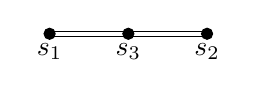
\begin{tikzpicture}
    \node at (-1,0) [below] {$s_{1}$};
    \node at (0,0) [below] {$s_{3}$};
    \node at (1,0) [below] {$s_{2}$};
    \draw (-1,0.03) -- (0,0.03) -- (1,0.03);
    \draw (-1,-0.03) -- (0,-0.03) -- (1,-0.03);
    \filldraw[black] (-1,0) circle (2pt);
    \filldraw[black] (0,0) circle (2pt);
    \filldraw[black] (1,0) circle (2pt);
  \end{tikzpicture}
\end{center}

Notice that upon identifying the $s_{1}$ and $s_{2}$ nodes and the $s_{3}$ and $s_{4}$ nodes respectively in $\wtilde{D_{4}}$, we recover the $\wtilde{C_{2}}$. This is a geometric realization of the fact that
\[
  Z(s_{1},s_{2},s_{3}) \quad \text{and} \quad Z_{\chi}(s_{1},s_{1},s_{2},s_{2},s_{3}),
\]
have similar symmetry properties. In \cite{DIPP}, a generalized Chinta-Gunnells action was described that can be used to build a multiple Dirichlet series $Z_{\wtilde{C_{2}}}(s_{1},s_{2},s_{3})$ whose group of functional equations is isomorphic to $\wtilde{C_{2}}$. This series is analogous to that of the role of $Z_{\wtilde{D_{4}}}(s_{1},\ldots,s_{5})$. In a 2014 thesis of Whitehead (see \cite{W}), it was shown that any multiple Dirichlet series satisfying a group of functional equations isomorphic to the affine Weyl group $W$, is determined by a unique series $Z_{W}$ up to a diagonal term when $W$ is \textit{simply laced}. This is because the functional equations induce recursive relations on the coefficients of the multiple Dirichlet series. If we impose additional growth conditions, then this diagonal term is $1$ and the series is necessarily $Z_{W}$. The root system of type $\wtilde{C_{2}}$ is not simply laced, yet the generalized Chinta-Gunnells action is amenable to the ideas presented in Whitehead's thesis. Accordingly, $Z_{\wtilde{C_{2}}}(s_{1},s_{2},s_{3})$ is the \textit{unique} series satisfying certain growth properties and a group of functional equations isomorphic to $\wtilde{C_{2}}$. This implies immediately that
\[
  Z_{\wtilde{C_{2}}}(s_{1},s_{2},s_{3}) = Z_{\wtilde{D_{4}}}(s_{1},s_{1},s_{2},s_{2},s_{3}),
\]
and therefore $Z_{\wtilde{C_{2}}}(s_{1},s_{2},s_{3})$ admits analytic continuation up to its natural barrier at $2s_{1}+2s_{2}+2s_{3} = -1$. The remaining question is how to express $Z(s_{1},s_{2},s_{3})$ in terms of $Z_{\wtilde{C_{2}}}(s_{1},s_{2},s_{3})$. Precisely, we are looking for an identity similar to \cref{equ:factorization}. To accomplish this, we expand $Z_{\wtilde{C_{2}}}(s_{1},s_{2},s_{3})$ into a Dirichlet series of shape
\[
  Z_{\wtilde{C_{2}}}(s_{1},s_{2},s_{3};q) = 1+\sum_{(k_{1},k_{2},k_{3}) \in \N^{3}-\{\mathbf{0}\}}a(k_{1},k_{2},k_{3};q)q^{-s_{1}k_{1}}q^{-s_{2}k_{2}}q^{-s_{3}k_{3}}.
\]
We at last define the multiple Dirichlet series
\[
  Z(s_{1},s_{2},s_{3}) = \sum_{m_{1},m_{2},d}\frac{a_{1}(m_{1})\chi_{d}(m_{1})a_{2}(m_{2})\chi_{d}(m_{2})A(m_{1},m_{2},d)}{|m_{1}|^{s_{1}}|m_{2}|^{s_{2}}|d|^{s_{3}}},
\]
where $a_{i}(m_{1})\chi_{d}(m_{i})$ are the coefficients of $L(s,E_{i} \x \chi_{d})$ and the coefficients $A(m_{1},m_{2},d)$ satisfy a twisted multiplicative property and are defined on primes by
\[
  A(p^{k_{1}},p^{k_{2}},p^{l}) = a\left(k_{1},k_{2},l;q^{-\frac{\deg(p)}{2}}\right). 
\]
We can apply the procedure in \cite{D} to sum up the series over $m_{1}$ and $m_{2}$ obtaining
\[
  Z(s_{1},s_{2},s_{3}) =  \sum_{d}\frac{L(s_{1},E_{1} \x \chi_{d})L(s_{2},E_{2} \x \chi_{d})P_{d}(s_{1},s_{2};E_{1},E_{2})}{|d|^{s_{3}}},
\]
where the correction polynomials $P_{d}(s_{1},s_{2};E_{1},E_{2})$ are now explicitly defined in terms of the $A(p^{k_{1}},p^{k_{2}},p^{l})$. This series satisfies a group of functional equations isomorphic to $\wtilde{C_{2}}$ where the functional equations are induced from those of $L(s_{i},E_{i} \x \chi_{d})$. Unfortunately, the analog of \cref{equ:factorization} is not so simple. The uniqueness theorem up to a diagonal established in \cite{W} only holds for $L$-functions with conductor $1$. The conductor of $L(s,E_{i} \x \chi_{d})$ is known to be at least quadratic. Nevertheless, the functional equations still induce recursive relations on the coefficients of the multiple Dirichlet series, but the recursive relations leave coefficients other than the diagonal coefficients undetermined. To state the relation, let $P_{+}$ be the set of positive weights and denote the integral basis of $P_{+}$ by $\{\w_{i}\}_{i}$. Set $\w = \sum\deg(N_{i})\w_{i}$. The analog of \cref{equ:factorization} has been verified to be of shape
\begin{equation}\label{equ:factorization_new}
  Z(s_{1},s_{2},s_{3}) = \sum_{\xi \in S_{\w}}F_{\w-\xi}(x^{-2s_{1}-2s_{2}-2s_{3}})x^{\w-\xi}Z_{\wtilde{C_{2}},\xi}(s_{1},s_{2},s_{3}),
\end{equation}
where $S_{\w} = \{\xi \in P:\xi \le \w\}$, the multiple Dirichlet series $Z_{\wtilde{C_{2}},\xi}$ is a twisted Chinta-Gunnells average, and the $F_{\w-\xi}$ are power series. The structure of $Z_{\wtilde{C_{2}},\xi}$ has been detailed in \cite{CFG} in the finite case and the extension to the affine case is expected to follow from \cite{W} in a similar way. The continuation of $Z_{\wtilde{C_{2}},\xi}$ to the natural barrier can then be deduced analogously to that for $Z_{\wtilde{C_{2}}}$. This reduces the analytic continuation of $Z$ to that of the factors $F_{\w-\xi}(x^{-2s_{1}-2s_{2}-2s_{3}})$. If we write,
\[
  F_{\w-\xi}(x) = \sum_{n \ge 0}a(n)x^{n},
\]
then $F_{\w-\xi}(x^{-2s_{1}-2s_{2}-2s_{3}})$ has continuation to the natural barrier if and only if $F_{\w-\xi}(x)$ converges for $|x| < 1$. This latter condition is determined entirely by the size of the coefficients $a(n)$ and we suspect $a(n) \ll n^{\e}$. This estimate is the essential barrier to the entire problem and is a type of \textit{Ramanujan-Petersson conjecture} for the series $F_{\w-\xi}(x)$. In the case $N_{1}$ and $N_{2}$ are quadratic, the coefficients $a(n)$ have a simple description and should be of the conjectured size. This will show that $F_{\w-\xi}(x^{-2s_{1}-2s_{2}-2s_{3}})$ converges up to the natural barrier and the continuation of $Z(s_{1},s_{2},s_{3})$ to the dead zone will follow from \cref{equ:factorization_new}.

\textbf{Broader Impacts}: There are a host of other investigations that may be conducted regarding different aspects of this problem and the strategies involved. In the following, we highlight two of the more urgent ones:

\begin{enumerate}
  \item The strategy to prove the simultaneous non-vanishing problem, involves finding an analogous asymptotic to \cref{equ:asymptotic}. This can be equivalently thought of as a \textit{first moment} result for the family $\{L\left(\frac{1}{2},E_{1} \x \chi_{d}\right)L\left(\frac{1}{2},E_{2} \x \chi_{d}\right)\}_{d}$. The shape of the main term of these moments for similar families has deep roots in random matrix theory. A classical example is the $r$-th moment of quadratic Dirichlet $L$-functions
  \[
      M_{r}(D) = \sum_{0 \le d \le D}L\left(\frac{1}{2},\chi_{d}\right)^{r}.
  \]
  It was conjectured
  \[
    M_{r}(D) \sim DQ(\log(D)),
  \]
  for some explicit polynomial $Q(x)$ of degree $\frac{r(r+1)}{2}$. Similar conjectures for other moments of various families of $L$-functions were studied by Conrey-Farmer-Keating-Rubinstein-Snaith. The infamous CFKRS conjectures (see \cite{CFKRS}) describe the main terms of these moments exactly by relating the statistical properties of families of $L$-functions to that of random matrices. It was conjectured by Diaconu-Goldfeld-Hoffstein, that there should exist additional lower order terms when $r \ge 3$. If $r = 3$, there should be one lower order term of $D^{\frac{3}{4}}$ and for $r \ge 4$, we have
  \[
    M_{r}(D) = \sum_{1 \le n \le N}D^{\left(\frac{1}{2}+\frac{1}{2n}\right)}Q_{n,r}(\log(D))+O(D^{\frac{1+\t}{2}}),
  \]
  for any $N \ge 1$ where $(N+1)^{-1} < \t < N$. The structure of the polynomials $Q_{n,r}$ was computed in \cite{DT} under some assumptions about analytic continuation. That is, there are infinitely many lower order terms. Moreover, \textbf{these lower order terms can only be detected via multiple Dirichlet series}. Since the first moment of $\{L\left(\frac{1}{2},E_{1} \x \chi_{d}\right)L\left(\frac{1}{2},E_{2} \x \chi_{d}\right)\}_{d}$ is structurally similar to the $4$-th moment of $\{L\left(\frac{1}{2},\chi_{d}\right)\}_{d}$ (this is the underpinning of the relationship between $Z_{\wtilde{C}_{2}}$ and $Z_{\wtilde{D_{4}}}$), similar methods in \cite{DT} are applicable. We therefore expect that the the first moment of $\{L\left(\frac{1}{2},E_{1} \x \chi_{d}\right)L\left(\frac{1}{2},E_{2} \x \chi_{d}\right)\}_{d}$ should exhibit infinitely many lower order terms. It would be very interesting to study the structure of these coefficients and compare them to those of $Q_{n,r}$ in \cite{DT}.

\item The CFKRS conjeture regarding the $r$-th moment of quadratic Dirichlet $L$-functions (over functional fields and with a minor restriction on $r$) was recently proven in a monumental paper by Bergstr\"om-Diaconu-Peterson-Westerland (see \cite{BDPW}) and and associated paper of Miller-Patzt-Petersen-Randal-Williams (\cite{MPPRW}). Precisely,
\[
  \frac{1}{q^{2g+1}}\sum_{\substack{d \text{ monic \& sq. free} \\ \deg(d) = 2g+1}}L\left(\frac{1}{2},\chi_{d}\right)^{r} = Q_{r}(2g+1)+o(1),
\]
provided $q$ is much larger than $r$. This is proved showing homological stability of the braid group with coefficients in a Schur functor applied to the integral reduced Burau representation. Upon computing the stable homology, the authors arrive at asymptotics for the traces of Frobenius on the \'etale (co)homology with coefficients in symplectic local
systems of the moduli space of smooth hyperelliptic curves of genus $g$ with a marked Weierstrass point. This asymptotic can be shown to be equivalent to the aforementioned CFKRS conjecture. This work is still being digested by many to understand the extent to which it can be generalized. However, since this is inherently an $r$-th moment problem, it is expected to generalize to $r$-th moments of families of $L$-functions indexed by quadratic twists. This means that one should be able to prove an analogous result for the family $\{L\left(\frac{1}{2},E_{1} \x \chi_{d}\right)L\left(\frac{1}{2},E_{2} \x \chi_{d}\right)\}_{d}$. As the Bergstr\"om-Diaconu-Peterson-Westerland method cannot detect lower order terms, (1) would be a strictly stronger result. However, it is the method of Bergstr\"om-Diaconu-Peterson-Westerland which is more interesting. Indeed, it is conjectured that the coefficients $a(n)$ in 
\[
  F_{\w-\xi}(x) = \sum_{n \ge 0}a(n)x^{n},
\]
when at least one of the conductors $N_{i}$ of $E_{i}$ is cubic, are obtained as traces of Hecke operators on spaces of automorphic forms. The description of the $a(n)$ however, are being packaged as character sums which are known to be point counting functions on the moduli spaces of curves. It is therefore possible that a proof of (1) using the Bergstr\"om-Diaconu-Peterson-Westerland method would provide additional information about the coefficients $a(n)$. In the best possible case, this would allow for the simultaneous non-vanishing result to hold when the conductors $N_{i}$ have arbitrarily large degree. A result of this form would be strictly stronger simultaneous non-vanishing result despite not being able to detect lower order terms.
\end{enumerate}

\begin{thebibliography}{}
  \bibitem{BDPW}
  Bergström, Jonas, et al. "Hyperelliptic curves, the scanning map, and moments of families of quadratic $L$-functions." arXiv preprint arXiv:2302.07664 (2023).

  \bibitem{BW}
  Friedberg, Solomon, ed. Multiple Dirichlet Series, Automorphic Forms, and Analytic Number Theory: Proceedings of the Bretton Woods Workshop on Multiple Dirichlet Series, Bretton Woods, New Hampshire, July 11-14, 2005. Vol. 75. American Mathematical Soc., 2006.

  \bibitem{CFKRS}
  Conrey, J. Brian, et al. "Integral moments of $L$-functions." Proceedings of the London Mathematical Society 91.1 (2005): 33-104.

  \bibitem{CFG}
  Chinta, Gautam, Solomon Friedberg, and Paul E. Gunnells. "On the $p$-parts of quadratic Weyl group multiple Dirichlet series." (2008): 1-23.

  \bibitem{Da}
  Davenport, Harold. Multiplicative number theory. Vol. 74. Springer Science \& Business Media, 2013.

  \bibitem{D}
  Diaconu, Adrian. "On the third moment of $L(\frac{1}{2},\chi_{d})$ I: The rational function field case." Journal of Number Theory 198 (2019): 1-42.

  \bibitem{DIPP}
  Diaconu, Adrian, et al. "Residues of quadratic Weyl group multiple Dirichlet series." arXiv preprint arXiv:2307.06223 (2023).

  \bibitem{DPP}
  Diaconu, Adrian, Vicentiu Pasol, and A. Popa. "Quadratic Weyl group multiple Dirichlet series of Type $D_{4}^{(1)}$." arXiv preprint arXiv:2111.11062.

  \bibitem{DT}
  Diaconu, Adrian, and Henry Twiss. "Secondary terms in the asymptotics of moments of $L$-functions." Journal of Number Theory 252 (2023): 243-297.

  \bibitem{GH}
  Goldfeld, Dorian, and Jeffrey Hoffstein. "Eisenstein series of $\frac{1}{2}$-integral weight and the mean value of real Dirichlet $L$-series." Inventiones mathematicae 80.2 (1985): 185-208.

  \bibitem{MPPRW}
  Miller, Jeremy, et al. "Uniform twisted homological stability." arXiv preprint arXiv:2402.00354 (2024).

  \bibitem{M}
  Murty, M. Ram, and V. Kumar Murty. Non-vanishing of $L$-functions and applications. Springer Science \& Business Media, 2012.

  \bibitem{W}
  Whitehead, Ian. Multiple Dirichlet series for affine Weyl groups. Columbia University, 2014.
\end{thebibliography}
\end{document}